\section{Chapter 1 -- Simple Linear Regression}


% ~~~~~~~~~~~~~~~~~~~~~~~~~~~~~~~~~~~~~~~~~~~~~~~~~~~~~~~~~~~~~~~~~~~~~~~
%      Subsection
% ~~~~~~~~~~~~~~~~~~~~~~~~~~~~~~~~~~~~~~~~~~~~~~~~~~~~~~~~~~~~~~~~~~~~~~~
\subsection{Overture}

\begin{figure}[H]
\caption{Okun's law in macroeconomics is an example of the simple linear regression. Here the dependent variable (GDP growth) is presumed to be in a linear relationship with the changes in the unemployment rate.}
\centering
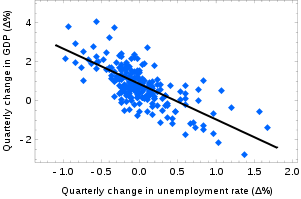
\includegraphics[width=3.3in]{images/okun.png}
\end{figure}


\begin{eq}{1.1.1 (SLR)} 
   $ y = \beta_0 + \beta_1x + \epsilon $
\end{eq}

\begin{as}{Model}
 \begin{enumerate}
     \item Each $y_i$ is a r.v. while each $x_i$ is a measured number.
     \item Each $\epsilon_i$ follows a normal distribution with mean 0 and variance $\sigma^2$
 \end{enumerate}
\end{as}
 
 
% ~~~~~~~~~~~~~~~~~~~~~~~~~~~~~~~~~~~~~~~~~~~~~~~~~~~~~~~~~~~~~~~~~~~~~~~
%      Subsection
% ~~~~~~~~~~~~~~~~~~~~~~~~~~~~~~~~~~~~~~~~~~~~~~~~~~~~~~~~~~~~~~~~~~~~~~~
\subsection{Model Fitting by Least Squares Method}
\begin{figure}[H]
\caption{The better the linear regression (on the right) fits the data in comparison to the simple average (on the left graph), the closer the value of $R^{2}$ is to 1. The areas of the blue squares represent the squared residuals with respect to the linear regression. The areas of the red squares represent the squared residuals with respect to the average value.}
\centering
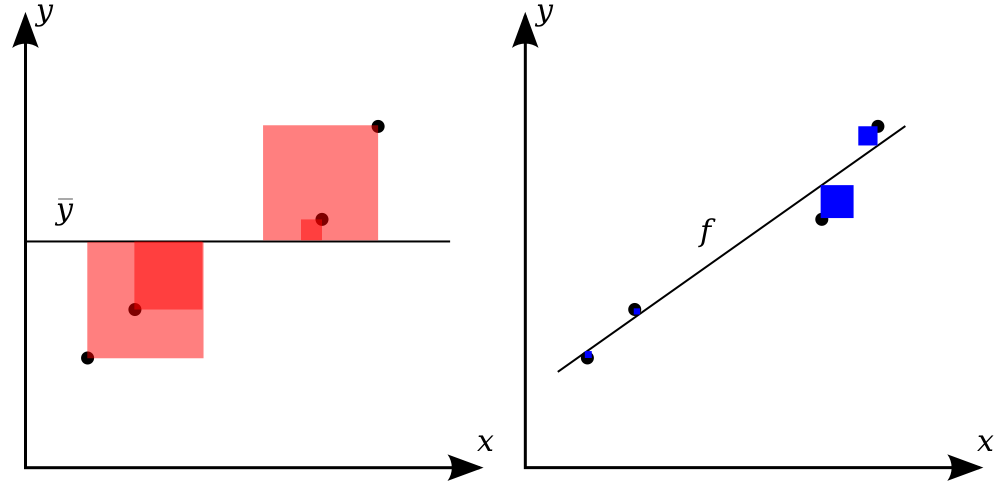
\includegraphics[width=3.3in]{images/R2.png}
\end{figure}


\begin{eq}{1.2.1 (Sum of squares)}
 $$ \mathrm{SS}(\beta_0, \beta_1) = \sum_{i=1}^{n} \big[ y_i - (\beta_0 + \beta_1 x_i) \big]^2  $$
\end{eq}

\begin{eq}{1.2.2 ($\beta_0$ and $\beta_1$)}
 $$ \hat{\beta_1} = \frac{S_{xy}}{S_{xx}} = \frac{\sum_{i=1}^n (x_i - \bar{x})(y_i - \bar{y})}{\sum_{i+1}^n (x_i - \bar{x})^2}  $$ 
 $$\hat{\beta_0} = \bar{y} - \hat{\beta_1}\bar{x}$$
 
 $$ S_{xy} := \sonen (x_i - \xbar)(y_i - \ybar) = \sonen x_i y_i - n \xbar\ybar \hspace{11pt}\mathrm{and} 
  \hspace{11pt} S_{xx} := \sonen (x_i - \xbar)^2 = \sonen x_i^2 - n\xbar^2 $$
\end{eq}

\begin{note}{Random errors and residuals}
    Random errors are unobservable random variables, whereas residuals are the measured errors.
\end{note}

\begin{fact}{Sum-to-zero constraints on residuals}
    \begin{enumerate}
         \item $\sonen e_i = 0$  provided that $\boneh  $ is included in the model.
         \item $\sonen x_ie_i = 0$
    \end{enumerate}
    These facts follow from the following equations surrounding least-squares optimization.
    
    $$ \frac{\partial}{\partial \beta_0 } \mathrm{SS} (\bzeroh,\boneh) = -2 \sonen [y_i - (\bzeroh + \boneh x_i )] = 0 $$
    $$ \frac{\partial}{\partial \beta_1 } \mathrm{SS} (\bzeroh,\boneh) = -2 \sonen x_i [y_i - (\bzeroh + \boneh x_i )] = 0 $$
\end{fact}

\begin{as}{Random error distribution}
     Note that each $\epsilon_i \sim N(0, \sigma^2) $ for some unknown variance $\sigma^2$. It's not necessary for least squares estimation, but it's crucial to much of the statistical inference and prediction which follow.
\end{as}


% ~~~~~~~~~~~~~~~~~~~~~~~~~~~~~~~~~~~~~~~~~~~~~~~~~~~~~~~~~~~~~~~~~~~~~~~
%      Subsection
% ~~~~~~~~~~~~~~~~~~~~~~~~~~~~~~~~~~~~~~~~~~~~~~~~~~~~~~~~~~~~~~~~~~~~~~~
\subsection{Assessing the Goodness of Fit of the Model}
\begin{figure}[H]
\caption{Comparison of the Theil--Sen estimator (black) and simple linear regression (blue) for a set of points with outliers. Because of the many outliers, neither of the regression lines fits the data well, as measured by the fact that neither gives a very high $R^2$.}
\centering
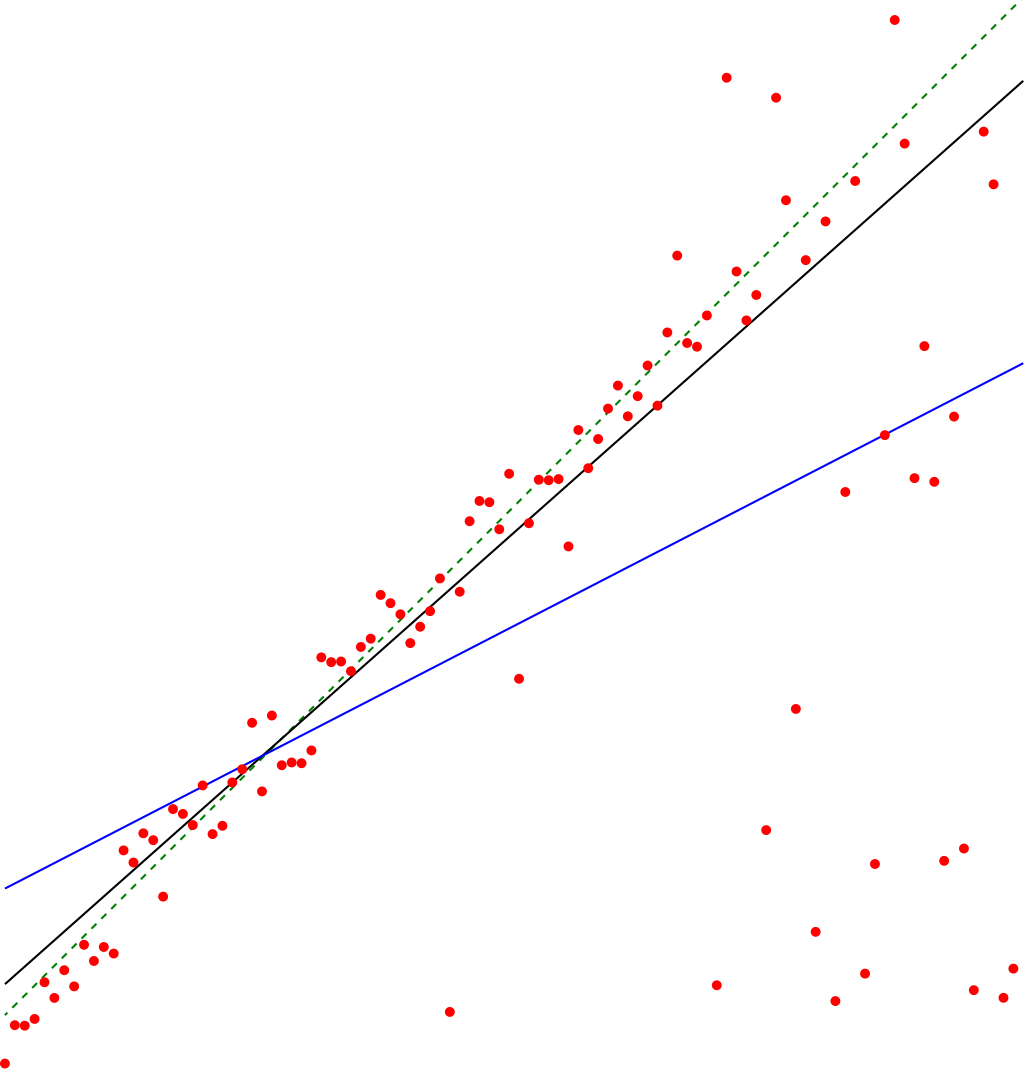
\includegraphics[width=3.3in]{images/thiel-sen.png}
\end{figure}


\begin{eq}{1.3.1 (Decomposition of sums of squares)}
     $$ \mathrm{TSS} = \mathrm{RSS} + \mathrm{Reg SS} $$
     $$ \sonen (y_i - \ybar)^2 = \sonen (y_i - \hat{y}_i)^2  + \sonen (\hat{y}_i - \ybar)^2 $$
\end{eq}

\begin{eq}{1.3.2 (Coefficient of determination)}
     $$ R^2 = \frac{\mathrm{Reg SS}}{\mathrm{TSS}} = 1 - \frac{\mathrm{RSS}}{\mathrm{TSS}} $$
\end{eq}

\begin{eq}{1.3.3 (Specialized formulas for RSS and Reg SS under SLR)}
     $$ \mathrm{Reg SS} = \boneh^2 S_{xx} $$
     $$ \mathrm{RSS} = \mathrm{TSS} - \mathrm{Reg SS} = S_{yy} - \boneh^2 S_{xx} $$
\end{eq}

\begin{eq}{(F-statistic)}
     $$\boxed{ F = \frac{\mathrm{Reg SS} / 1}{\mathrm{RSS} / (n-2)} }$$
\end{eq}

\begin{fact}{Consequences of the specialized formulas for Reg SS and RSS}
    \begin{enumerate}
        \item The regression sum of squares is directly proportional to the square of the least
        squares estimator of the slope parameter.
        \item In an SLR model, the coefficient of determination is simply the sample correlation between X and Y.
    \end{enumerate}
\end{fact}

\begin{fact}{Unbiased estimator of error variance}
    $$ \mathrm{MSE} = s^2 = \frac{\mathrm{RSS}}{n-2} = \frac{\sonen e_i^2}{n-2} $$
Here the MSE can be shown to be an unbiased estimator of the unknown error variance, $\sigma^2$. The residual standard deviation, or residual standard error, or RSE, is simply the square root of the MSE.
\end{fact}

\begin{eq}{1.3.4 (F-statistic in terms of $R^2$)}
    $$ F = (n-2) \frac{R^2}{1-R^2} $$  \hspace{288pt}(using the divide by TSS trick)
\end{eq}


% ~~~~~~~~~~~~~~~~~~~~~~~~~~~~~~~~~~~~~~~~~~~~~~~~~~~~~~~~~~~~~~~~~~~~~~~
%      Subsection
% ~~~~~~~~~~~~~~~~~~~~~~~~~~~~~~~~~~~~~~~~~~~~~~~~~~~~~~~~~~~~~~~~~~~~~~~
\subsection{Statistical Inference about Regression Coefficients -- Hypothesis Tests and Confidence Intervals}
\begin{figure}[H]
\caption{In this bar chart, the top ends of the brown bars indicate observed means and the red line segments ("error bars") represent the confidence intervals around them. Although the error bars are shown as symmetric around the means, that is not always the case. It is also important that in most graphs, the error bars do not represent confidence intervals (e.g., they often represent standard errors or standard deviations)}
\centering
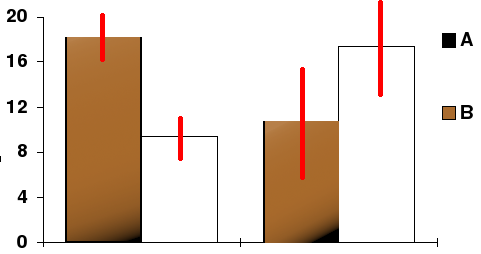
\includegraphics[width=3in]{Confidenceinterval.png}
\end{figure}


\begin{eq}{1.4.1 and 1.4.2 (Estimated variances of $\boneh$ and $\bzeroh$)}
    $$ \widehat{\mathrm{Var}}(\bzeroh) = s^2 \bigg( \frac{1}{n} + \frac{\xbar^2}{S_{xx}} \bigg) = \frac{s^2 \sonen x_i^2}{nS_{xx}} \hspace{11pt}\mathrm{and}\hspace{11pt}\widehat{\mathrm{Var}}(\boneh) = \frac{s^2}{S_{xx}}$$
    Note that the standard errors of the estimated best-fit parameters are simply the square roots of the estimated variances.
\end{eq}

\begin{eq}{($t$ Statistic)}
    $$ t(\hat{\beta}_j ) = \frac{\hat{\beta}_j  - \beta_{j, H_0}}{\mathrm{SE}(\hat{\beta}_j )} $$
    $$ t(\hat{\beta}_j ) \sim t_{n-2} $$ under $H_0$
\end{eq}

\begin{eq}{(Confidence Interval for LSEs)}
$$ \textnormal{Confidence Interval} = \mathrm{LSE} \pm \textnormal{t-quantile} \cdot \mathrm{SE} = \hat{\beta}_j \pm t_{n-2,\alpha/2} \cdot \textnormal{SE}(\hat{\beta}_j ) $$
\end{eq}


\begin{eq}{(Relationship between $t$ and $F$)}
$$ t(\boneh)^2 = \frac{\boneh^2}{s^2/S_{xx}} = \frac{\boneh^2 S_{xx}}{s^2} = \frac{\mathrm{Reg SS}/1}{\mathrm{RSS}/(n-2)} = F $$
\end{eq}


% ~~~~~~~~~~~~~~~~~~~~~~~~~~~~~~~~~~~~~~~~~~~~~~~~~~~~~~~~~~~~~~~~~~~~~~~
%      Subsection
% ~~~~~~~~~~~~~~~~~~~~~~~~~~~~~~~~~~~~~~~~~~~~~~~~~~~~~~~~~~~~~~~~~~~~~~~
\subsection{Prediction}
\begin{figure}[H]
\caption{Prediction interval (on the y-axis) given from z (the quantile of the standard score, on the x-axis). The y-axis is logarithmically compressed (but the values on it are not modified).}
\centering
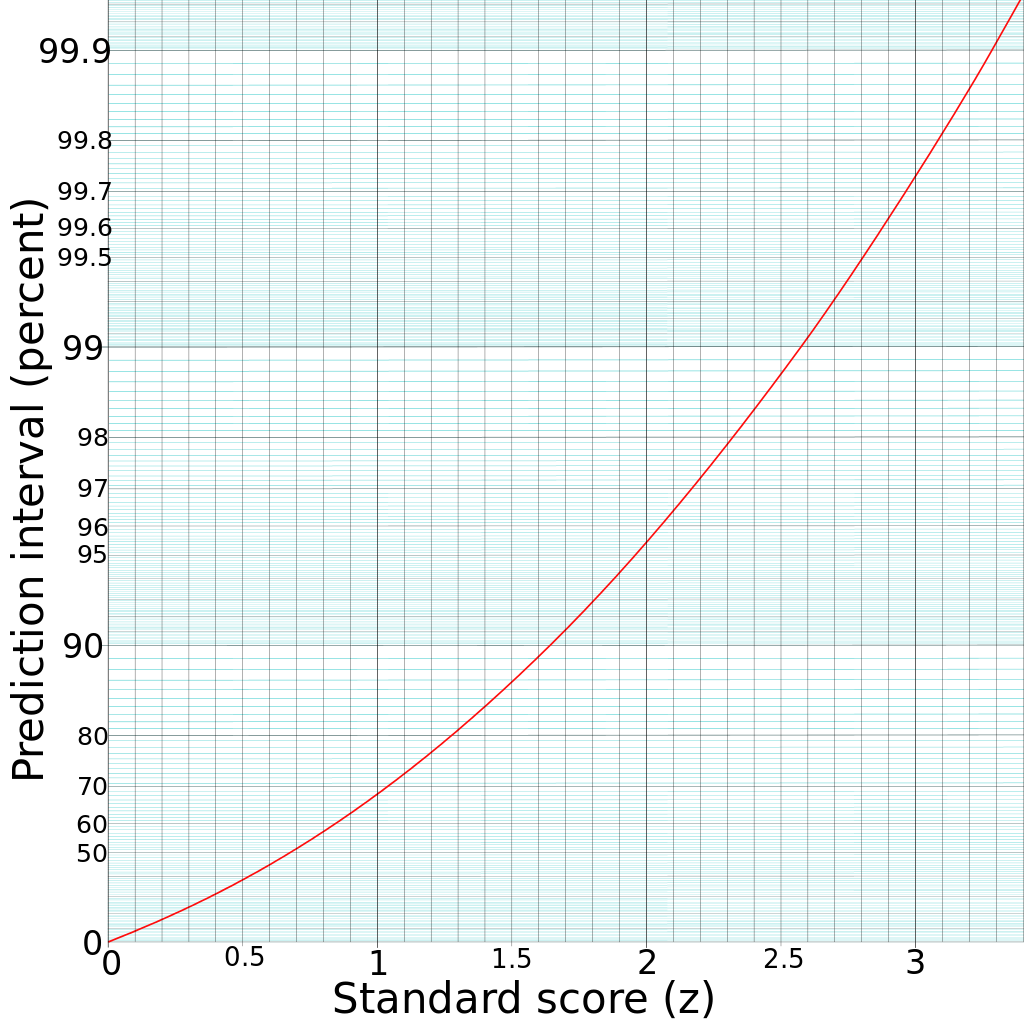
\includegraphics[width=3in]{PI.png}
\end{figure}

\begin{eq}{1.5.2 (Prediction intervals)}
$$ \hat{y}_* \pm t_{n-2, \alpha/2}
\cdot \mathrm{SE}(y_* - \hat{y_*}) = 
(\bzeroh + \boneh x^*) \pm t_{n-2, \alpha/2} 
\sqrt{s^2 \bigg[  1 + \frac{1}{n} + \frac{(x^* - \xbar)^2}{S_{xx}} \bigg]} $$
\end{eq}


% ~~~~~~~~~~~~~~~~~~~~~~~~~~~~~~~~~~~~~~~~~~~~~~~~~~~~~~~~~~~~~~~~~~~~~~~
%      Subsection
% ~~~~~~~~~~~~~~~~~~~~~~~~~~~~~~~~~~~~~~~~~~~~~~~~~~~~~~~~~~~~~~~~~~~~~~~
\subsection{Problems}
\begin{eq}{1.6.1 ($\boneh$ in terms of $r$)}
$$ \boneh = r \cdot \frac{\sy}{\sx} $$ \vspace{19pt}
\hspace{261pt} where $\sx = \sqrt{\sxx/(n-1)}$ and \\
.\hspace{271pt}$\sy = \sqrt{\syy/(n-1)}$
\end{eq}

% left off on 1.6.33